\chapter{Evaluierung des Open API 2.0 Plugins von OWASP ZAP}
\label{cha:k5}

Die in Abschnitt \ref{ablaufpentest} vorgestellten Schritte eines Penetrationstests werden in diesem Kapitel zur Evaluierung des Open API 2.0 Plugins von OWASP ZAP herangezogen. Um die bereits entwickelte Spring Boot Anwendung auf Sicherheitslücken zu testen, werden mit Hilfe des Open API 2.0 Plugins von OWASP ZAP die Penetrationstests durchgeführt.

\section{Ablauf des Open API 2.0 Plug-In von OWASP ZAP}

\subsection{Vorbereitung}

In der Vorbereitungsphase werden die entsprechenden Anforderungen für einen Penetrationstest erfüllt, um eine sichere Anwendung zu entwickeln. Hier wird bestimmt, welche Komponenten dem Test unterzogen werden. Mittels \texttt{Spring Boot} kann automatisiert eine Dokumentation der REST-API als \texttt{Swagger 2.0} generiert werden. Die automatisch generierten \texttt{REST Docs} werden in das \texttt{OpenAPI 2.0} Plugin von OWASP ZAP importiert und die geeigneten REST-API-Sicherheitstests werden für die Schwachstellen durchgeführt. Außerdem kann dieser Penetrationstest in das Konzept des White-Box-Tests eingestuft werden, da vollständige Kenntnisse der zu testenden Infrastruktur vorliegen.

\subsection{Informationsbeschaffung}

Nach Abschluss der Vorbereitungsphase kann die Beschaffung von Information über die Spring Boot Anwendung erfolgen. Diese ist im Online-Shop verfügbar und enthält bestimmte Produkte. Durch die REST-API können Produkte aufgerufen, angezeigt, hinzugefügt, aktualisiert und gelöscht werden. In der Regel wird ein Portscan gegen das Zielsystem durchgeführt, um einen Überblick zu erlangen, welche Dienste erreichbar sind. Doch in diesem Fall wird Portscan nicht benötigt, weil automatisch durch das \texttt{OpenAPI 2.0} Plugin alle erreichbaren Dienste aufgerufen werden können. Zusätzlich ist zu erwähnen, dass bereits bekannt ist, welche Funktionalitäten diese Spring Boot Anwendung besitzt, weshalb in dieser Phase nicht viel Zeit zu investieren ist.

\subsection{Bewertung der Informationen und Risikoanalyse}

In der vorherigen Phase wurden alle notwendigen Informationen gesammelt, die in dieser Phase ausführlich zusammengetragen werden. Da der Autor dieser Arbeit die Spring Boot Anwendung selbst entwickelt hat, wird OWASP ZAP im \texttt{Attack Mode} Penetrationstests durchgeführt, damit kein rechtliches Problem auftritt. \texttt{Attack Mode} bedeutet, dass noch mehr unnötige Informationen in das Programm geladen werden. Deshalb ist es wahrscheinlicher, dass das Programm beschädigt wird und danach eventuell nicht alle Funktionalitäten erfüllen kann.

\subsection{Aktive Eindringversuche}

Laut der Risikoanalyse in der dritten Phase können die Penetrationstests für die REST-API durchgeführt werden. Durch das \texttt{OpenAPI 2.0} Plugin von OWASP ZAP wird in die Spring Boot Anwendung so weit wie möglich vorgedrungen. Da durch den Versuch einzudringen die Spring Boot Anwendung beschädigt werden kann, wird nun ein Schattensystem (eine exakte Kopie des zu testenden Systems) verwendet.\\

\newpage

\begin{figure}[h]
	\centering
	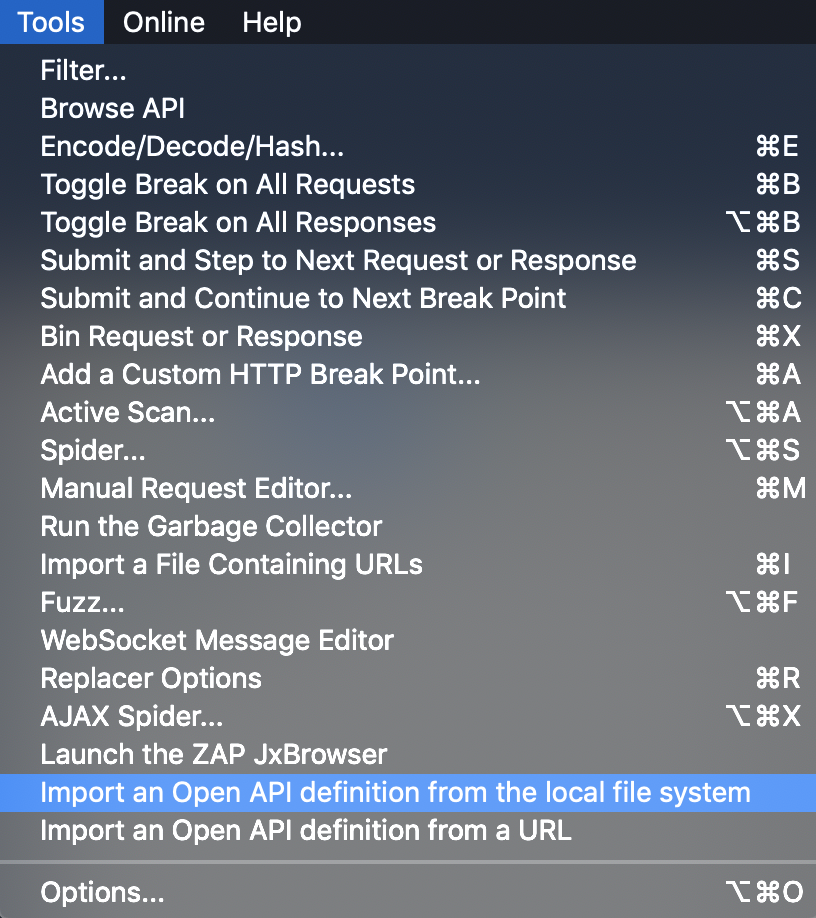
\includegraphics[width=8cm]{2-importbuttonoa2.png}
	\caption{Menuleiste des Open API Plugins}
	\label{swaggerimport1}
\end{figure}

Um den REST-API-Penetrationstest durchzuführen, wird von der Menüleiste \texttt{Tools} geklickt und danach wird \texttt{Import an Open API definition from the local file system} wie bei der \ref{swaggerimport1} gewählt.

\begin{figure}[h]
	\centering
	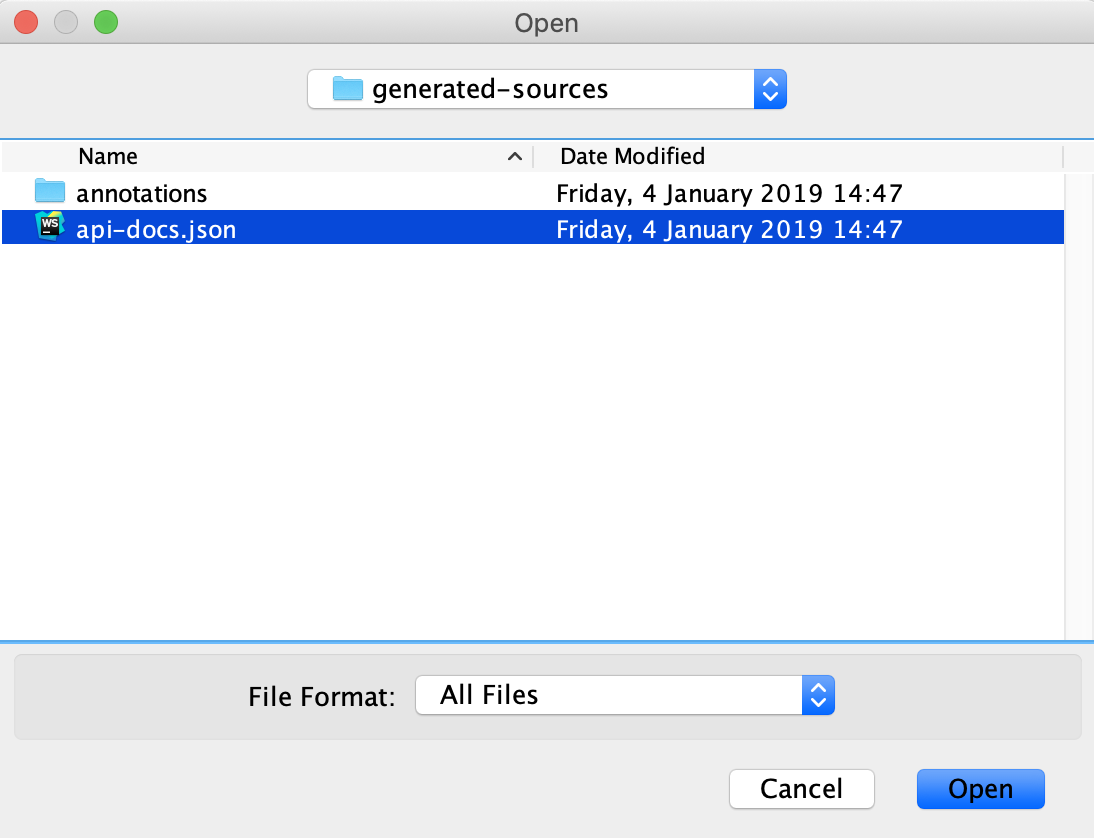
\includegraphics[width=8cm]{3-swaggerfilefortest.png}
	\caption{Importieren von Swagger 2.0 Datei}
	\label{swaggerimport2}
\end{figure}


Wie in der Abbildung \ref{swaggerimport2} erkennbar, wird die lokale Swagger 2.0 Datei ins OWASP ZAP durch das OpenAPI 2.0 Plugin importiert.

\begin{figure}[h]
	\centering
	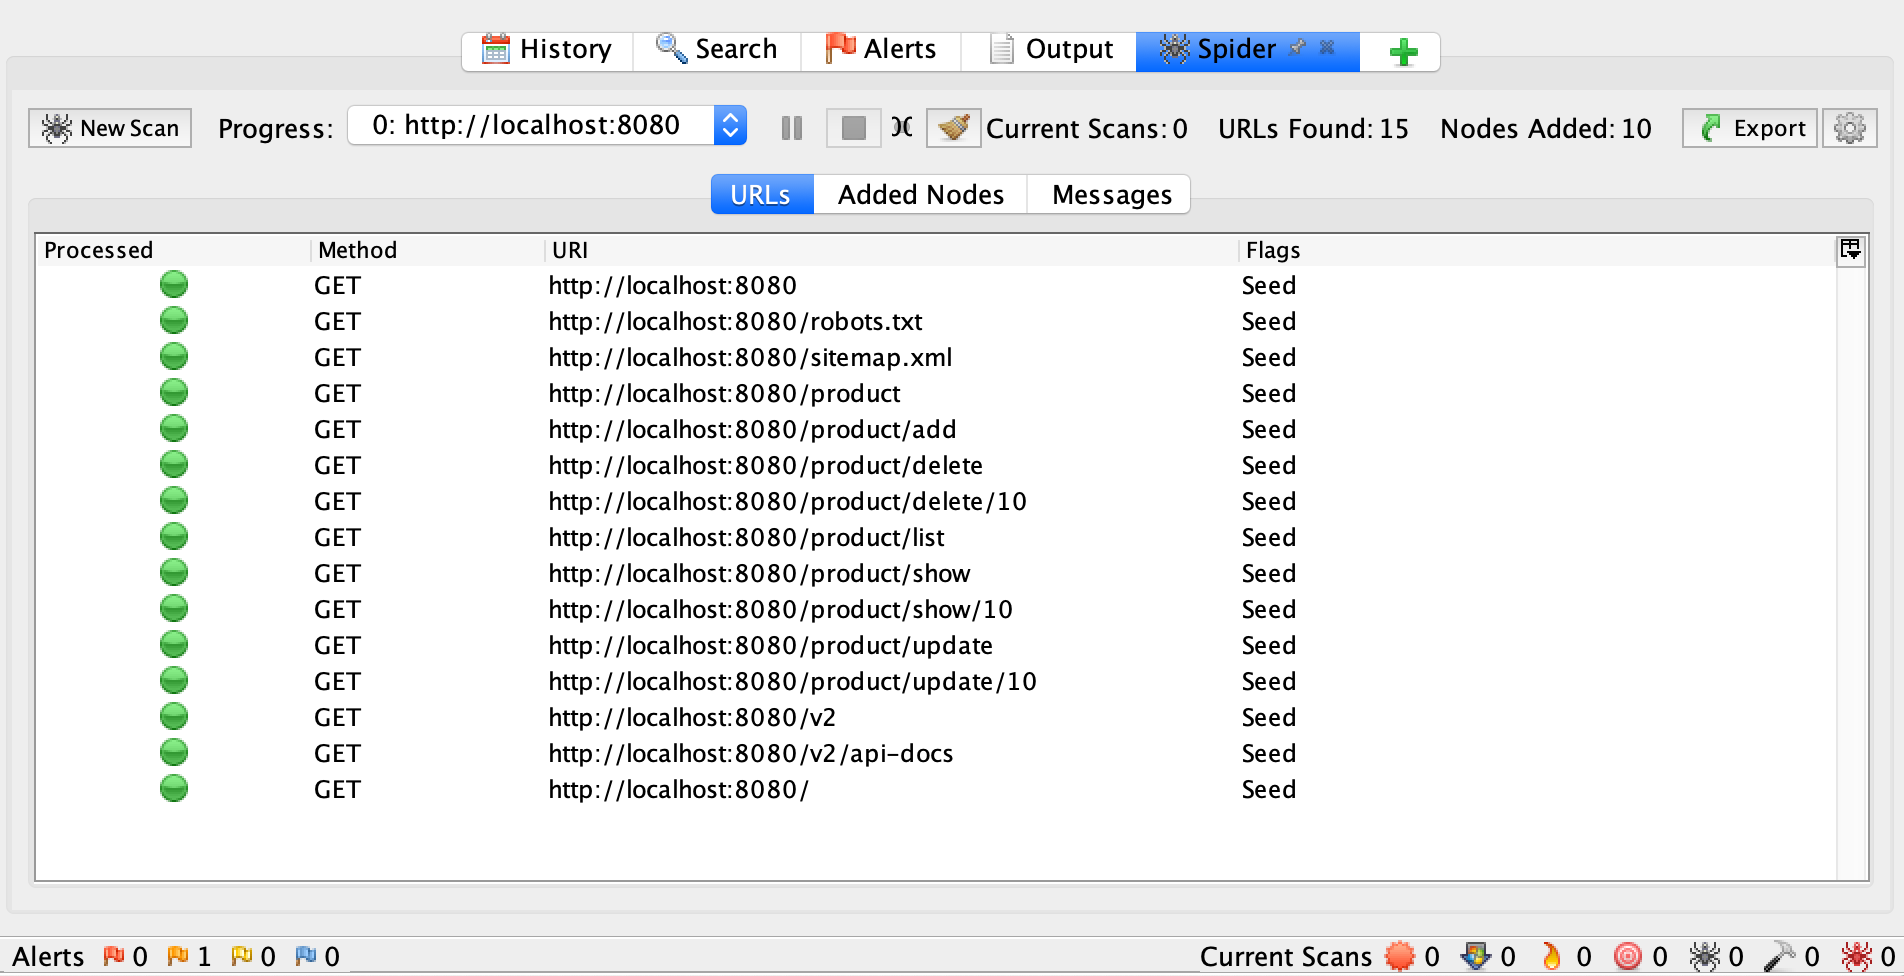
\includegraphics[width=14cm]{5-spiderofurls}
	\caption{Auflistung von erreichbare Diensten}
	\label{swaggerimport3}
\end{figure}

Danach werden durch den Spider alle möglichen Links aufgelistet (siehe \ref{swaggerimport3}), wenn diese erreichbar sind. Nun kann mit dem Active Scan wie in Abbildung \ref{swaggerimport4} gestartet werden. 

\begin{figure}[h]
	\centering
	\includegraphics[width=14cm]{6-activescancall.png}
	\caption{Aufrufen von Active Scan}
	\label{swaggerimport4}
\end{figure}

Während des Active-Scan-Fortschritts wird die lokal laufende Spring Boot Anwendung auf Sicherheitslücken wie SQL-Injektion, Buffer Overflow, XSS usw. geprüft.

\newpage

Wenn die Suche nach Sicherheitslücken erfolgreich beendet ist, werden alle gefundenen Sicherheitslücken (siehe Abbildung \ref{swaggerimport5} angezeigt.

\begin{figure}[h]
	\centering
	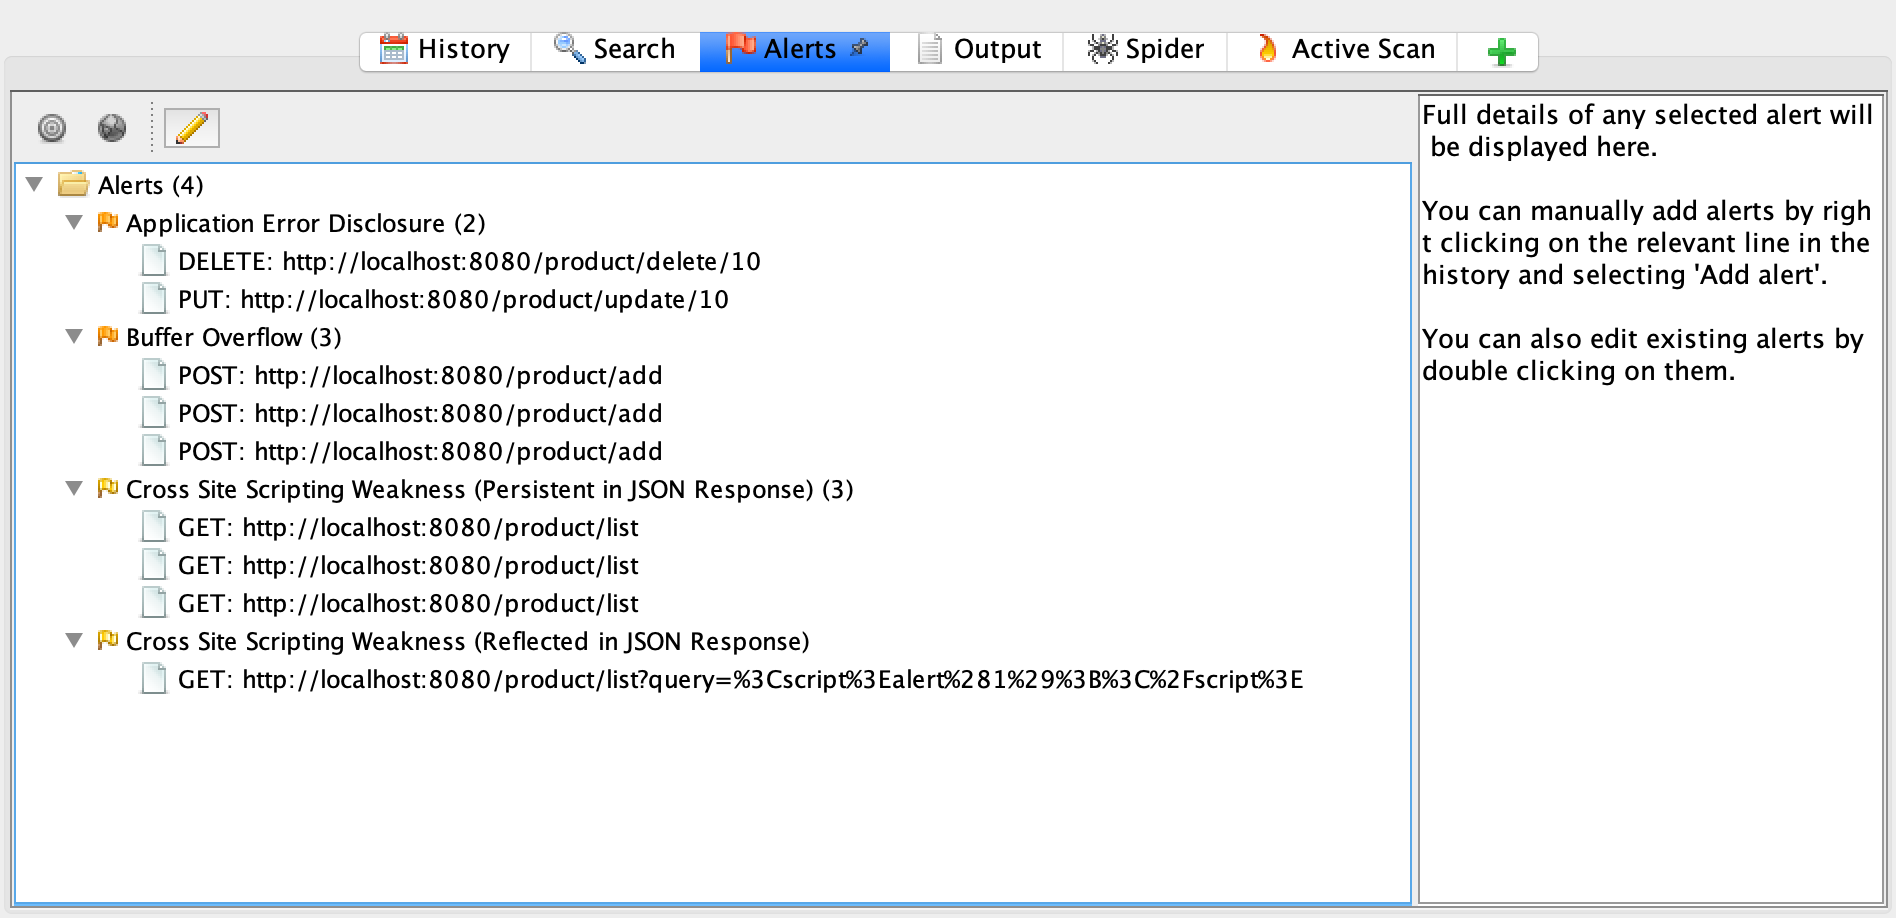
\includegraphics[width=12cm]{7-scanergebnis.png}
	\caption{Ergebnis des Active Scan}
	\label{swaggerimport5}
\end{figure}

\subsection{Abschlussanalyse}

Nach dem Ergebnis des OWASP ZAPs wurden die folgenden Sicherheitslücken gefunden:

\begin{itemize}
	\item Application Error Disclosure (2 Stück)
	\item Buffer Overflow (3 Stück)
	\item Cross Site Scripting Weakness (Persistent in JSON Response) (3 Stück)
	\item Cross Site Scripting Weakness (Reflected in JSON Responses)
\end{itemize}

\subsubsection{Vermeidung von Application Error Disclosure}

Wenn eine Anwendung einem Benutzer einen Fehler anzeigt, sollte eine Fehlernachricht die Ursache des Fehlers erklären können. Durch eine normale Stack Trace kann ein Angreifer zusätzliche Informationen über das System erfahren.

Wenn ein Benutzer z. B. aus Versehen (oder absichtlich) ein \texttt{\&} in ein Inputfeld eingibt, muss die Anwendung anstelle der vollständigen Fehlerdetails aufgrund der Programmierlogik die Meldung \texttt{Fehler aufgrund nicht unterstützter Zeichen. Überprüfen Sie Ihre Eingabe} anzeigen\cite{ase17}.

\subsubsection{Vermeidung von Buffer Overflow}

Webanwendungen oder Webdienste verwenden Eingaben aus HTTP-Anforderungen (und gelegentlich Dateien), um zu bestimmen, wie sie reagieren sollen. Angreifer können jeden Teil einer HTTP-Anfrage manipulieren, einschließlich der URL, der Abfragezeichenfolge, der Header, der Cookies, der Formularfelder und der ausgeblendeten Felder, um die Sicherheitsmechanismen der Seite zu beschädigen. Der verbreitete Angriff für einen Manipulationsangriff ist der Pufferüberlauf.

Der Server sollte niemals annehmen, dass der Content-Type immer den Inhaltstyp-Header und den Inhalt desselben Typs überprüft. Ein Mangel an Content-Type-Headern oder unerwarteten Content-Type-Headern sollte dazu führen, dass der
Server den Inhalt mit einer Antwort \texttt{406 Not Acceptable} ablehnt\cite{bofangpre16}.

\subsubsection{Vermeidung von Cross Site Scripting (Persistent)}

Um Persistent XSS am besten zu verhindern, muss sichergestellt werden, dass alle Benutzereingaben ordnungsgemäß bereinigt werden, bevor sie dauerhaft auf dem Webserver gespeichert werden. Außerdem müssen die statischen Inhalte, die den Benutzern angezeigt werden, ebenfalls bereinigt werden\cite{xsspersistent14}.

\subsubsection{Vermeidung von Cross Site Scripting (Reflected)}

Web Application Firewalls (WAF) haben eine bedeutende Funktion bei der Abwehr reflektierter XSS-Angriffe. Mit signaturbasierten Sicherheitsregeln kann eine WAF das Fehlen von Eingabebereinigungen ausgleichen und abnormale Anforderungen blockieren. Dies umfasst Anforderungen, die versuchen, einen reflektierten Cross-Site-Scripting-Angriff auszuführen\cite{xssreflected16}.

\newpage

\section{Bedeutung des automatisierten API-Penetrationstesting}

\begin{quote}
	\emph{\\
		"`Design all API security with public access in mind"'}
	\begin{flushright}
		Phillipp Schöne, Axway
	\end{flushright}
\end{quote}

Der Hauptgrund ist für die Größe der API-Angriffsflächen ist, dass die Webanwendungen in \texttt{micro-services} aufgeteilt werden, wodurch eine große Anzahl von Schnittstellen entstehen und diese dem öffentlichen Internet zugänglich gemacht werden. Dadurch werden zahlreiche Angriffsflächen erstellt, sodass Hacker nicht mehr eine einzelne Anwendung angreifen müssen. Sie können sich eine Vielzahl von Diensten ansehen, wodurch das Risiko erhöht wird, dass sie auf Daten zugreifen können\cite{mswv17}. 

Im Vergleich zu anderen Komponenten ist die API in einer Anwendung die schwächste Verbindung, die ein Hacker nach Datenverletzungen suchen kann. API-Sicherheitstests gewährleisten, dass die API vor Schwachstellen geschützt ist. Der API-Hack einer Anwendung kann Verwirrung auf Organisationsebene verursachen und zu erheblichen Verlusten für eine Organisation führen [16]. Des Weiteren besteht das größte Problem bei der API- und Micro-Services-Sicherheit derzeit darin, dass sie häufig als nachträglicher Vorgang und nicht als wesentlicher Bestandteil des Entwicklungsprozesses\cite{anthonyart18}.

Wenn mit dem Entwickeln der API-Sicherheitstests bis nach der Entwicklung gewartet wird, werden sie so vorbereitet, dass nur die günstigen Testfälle durchgeführt werden. Sobald eine API oder ein Teil der Software erstellt wurde, wird darauf geachtet, wie sie funktioniert werden soll, aber es werden nicht die anderen wahrscheinlichen Szenarien berücksichtigt. Dagegen werden die Penetrationstests durch das OpenAPI Plugin von OWASP ZAP während der Entwicklung durchgeführt und mit Hilfe dieser Situation werden API-Tests stärker und umfassender. Dies kommt dem Team langfristig zugute, da sich die API-Qualität erhöht und die Anzahl der aufgetretenen Fehler verringert wird. Die Erfassung aller Grundlagen potenzieller Softwarefehler ist eine entscheidende Komponente für die Aufrechterhaltung des Qualitäts- und Kundenvertrauens. Automatisierte API-Tests während der Entwicklung können Probleme mit der API, dem Server, anderen Diensten oder dem Netzwerk aufdecken, die nach der Bereitstellung möglicher-weise nicht einfach gefunden oder gelöst werden können. Sobald die Software in der Produktion ist, werden durch OWASP ZAP manuelle Tests erstellt, um neue und weiterentwickelte Anwendungsfälle zu testen. Restful-API-Tests können auf verschiedene Arten in den Entwicklungsprozess integriert werden. API-Testings in Continuous Integration und Continuous Deployment werden von diversen Unternehmen in ihren jeweiligen Prozessen angeboten. Wenn ein API-Test während CI oder CD fehlschlägt, wird der Prozess angehalten und das API-Problem muss behoben werden, bevor der Build abgeschlossen ist. Die Benutzung des OpenAPI Plugins von OWASP ZAP für automatisierte API-Tests in diesem Prozess gibt den Entwicklern mehr Sicherheit, dass alle Grundlagen vor der Veröffentlichung des Produkts für die Kunden erfüllt werden\cite{restcaseapiimportance16}.
